%\documentclass[a4paper]{article}
\usepackage[utf8]{inputenc}
\usepackage[spanish, es-tabla, es-noshorthands]{babel}
\usepackage[table,xcdraw]{xcolor}
\usepackage[a4paper, footnotesep = 1cm, width=20cm, top=2.5cm, height=25cm, textwidth=18cm, textheight=25cm]{geometry}
%\geometry{showframe}

\usepackage{tikz}
\usepackage{amsmath}
\usepackage{amsfonts}
\usepackage{amssymb}
\usepackage{float}
\usepackage{graphicx}
\usepackage{caption}
\usepackage{subcaption}
\usepackage{multicol}
\usepackage{multirow}
\setlength{\doublerulesep}{\arrayrulewidth}
\usepackage{booktabs}
\usepackage{mathrsfs,amsmath}
\usepackage{hyperref}
\hypersetup{
    colorlinks=true,
    linkcolor=blue,
    filecolor=magenta,      
    urlcolor=blue,
    citecolor=blue,    
}

\newcommand{\quotes}[1]{``#1''}
\usepackage{array}
\newcolumntype{C}[1]{>{\centering\let\newline\\\arraybackslash\hspace{0pt}}m{#1}}
\usepackage[american]{circuitikz}
\usetikzlibrary{calc}
\usepackage{fancyhdr}
\usepackage{units} 

\graphicspath{./Imagenes}

\pagestyle{fancy}
\fancyhf{}
\lhead{22.05 ASSD}
\rhead{Mechoulam, Lambertucci, Rodriguez, Londero}
\rfoot{Página \thepage}

%\begin{document}
\definecolor{turquoise}{rgb}{0, 0.68627,0.68627}
\definecolor{caribbeangreen}{rgb}{0.0, 0.8, 0.6}
\subsection{Sample and Hold}

El modulo de \textbf{Sample and Hold}  puede ser esquematizado de la siguiente forma:

\begin{figure}[H]
	\centering
	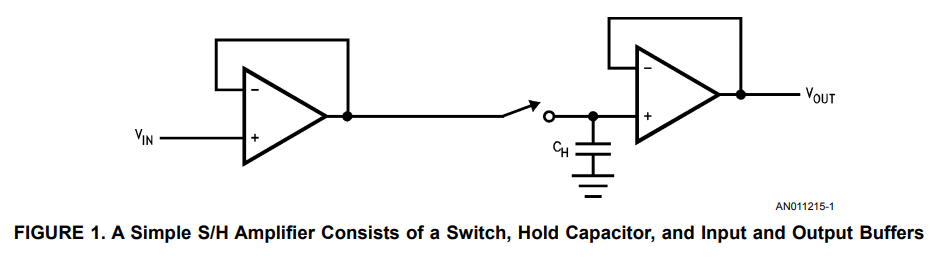
\includegraphics[width=0.7\linewidth]{ImagenesEjercicio4/SyH}
	\caption{}
	\label{fig:syh}
\end{figure}
Su objetivo es el de muestrear la señal analógica de entrada y retener su valor por un pequeño intervalo de tiempo para que la circuiteria colocada inmediatamente después puede utilizar ese valor para digitalizarla.
\subsubsection{Breve introducción formal al muestreo de señales con Sample and Hold}
Dada una señal analógica de entrada $x_{a}(t)$ deseamos obtener una señal discreta $x(n)$ producto de muestrar la entrada cada $T$ segundos.
Como primer paso para hallar la expresión que describe a la señal discreta efectuamos un muestreo ideal sobre la entrada

\begin{equation}
	\centering
	x_{\delta_{T}}(n)=\sum_{-\infty}^{\infty} x_{a}(t)\delta_{T}(t-nT)
	\label{
		muestreo_ideal}
\end{equation}
$$x_{\delta_{T}}(n) =x_{a}(nT) $$
Una vez tomadas las muestras de la señal, la convolucionaremos con un pulso unitario de duración $T$


$$x(n)=p(t)*\sum_{-\infty}^{\infty} x_{a}(nT)\delta_{T}(t-nT)$$
\begin{equation}
\centering
x(n)=\sum_{-\infty}^{\infty} x_{a}(nT)p_{T}(t-nT)
\end{equation}

Este proceso queda ilustrado en la figura \ref{fig:sh-circuit-waveform}
\begin{figure}[H]
	\centering
	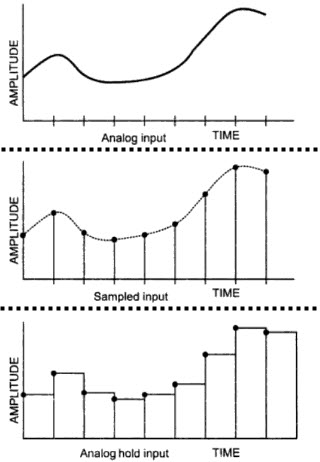
\includegraphics[scale=0.5]{ImagenesEjercicio4/SH-Circuit-Waveform}
	\caption{}
	\label{fig:sh-circuit-waveform}
\end{figure}

\subsubsection{Consideraciones sobre el modulo Sample and Hold}
Para esto, requerimos de una alta impedancia de entrada lo cual evita cualquier efecto de carga del IC sobre la fuente de la señal. Esto es modelado como un buffer a la entrada. Luego tenemos una \textbf{llave}, que puede estar implementada con una llave analogica o transistores MOSFET, la cual se encargara de cambiar del modo muestreo (sample) permitiendo que el capacitor se carga con el valor actual, y mantener (hold) ese valor cuando la misma este abierta. Finalmente tenemos un buffer adicional a la salida para prevenir la descarga del capacitor y así ofrecer mayor fidelidad. 


 Sin embargo, es necesario adaptarlo a las condiciones en las que se lo va a utilizar. Para esto, se incluyen pines de corrección de tensión de offset, selección tasa de muestreo (para controlar la "llave") y finalmente otro muy importante para escoger el capacitor, $C_{hold}$ más apropiado.
 Es interesante mencionar la inclusión de un pin \textbf{LOGIC REFERENCE} el cual nos brinda mayor flexibilidad al momento de tener que elegir una señal de muestreo
 %\footnote{Para saber más sobre el funcionamiento y puesta a punto del LF398 revisar el apéndice A}.
 \subsubsection{Circuito de corrección de tensión offset}
 Para poder obtener una digitalización de alta fidelidad es necesario calibrar el IC. En el caso de la digitalización de señales las tensiones de offset pueden provocar interpretaciones erróneas de los verdaderos valores de la señal. De hecho se recomienda que la tensión de offset este por debajo de la mitad del voltaje que ofrece el LSB.
 $$
 V_{OS} < \frac{FS}{2^{n+1}} 
 $$
Donde \textit{n }es la resolución del \textbf{ADC}
y \textit{FS} es el tope de escala.
Asumiendo un que los rangos de señal pueden variar entre $\pm15$ nos da una $FS=30$.
$$V_{OS}<\frac{FS}{2^{n+1}}$$
$$V_{OS}<\frac{30V}{2^{8+1}}$$
$$V_{OS}<58.5mV$$
El fabricante nos brinda una configuración para poder compensar la tensión de offset tanto de AC como de DC:
\begin{figure}[H]
	\centering
	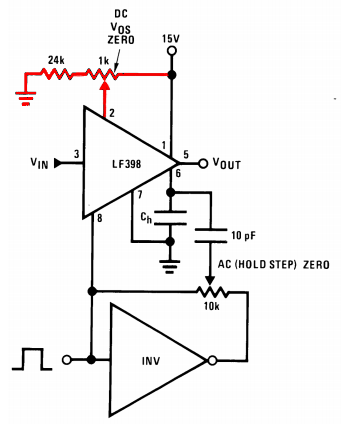
\includegraphics[scale=0.6]{ImagenesEjercicio4/DCcolorized}
	\caption{En \textcolor{red}{rojo} se señala el circuito de corrección de tensión DC, en la parte inferior notamos la presencia de un circuito que corrige la señal AC no deseada}
	\label{fig:dccolorized}
\end{figure}
Para poder establecer la necesidad o no de tener que utilizar el circuito de compensación hemos de medir la tensión de offset:
\begin{figure}[H]
	\centering
	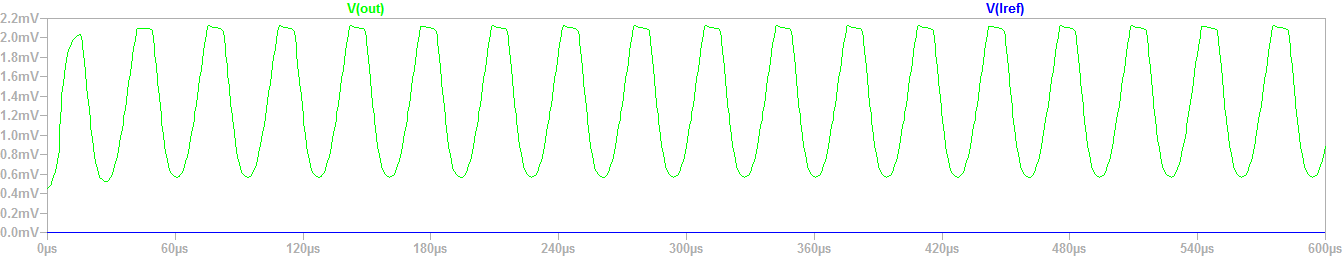
\includegraphics[width=\linewidth]{ImagenesEjercicio4/DCACoffset}
	\caption{Offset de DC y AC con entrada nula}
	\label{fig:dcacoffset}
\end{figure}
Del gráfico concluimos:
$$V_{offset DC}\approx 1mV$$
$$V_{offset AC}\approx 2mV_{pp}$$

Dado que el offset indeseado no supera el limite permitido podemos prescindir del uso de los circuitos de ajuste.

\subsubsection{Análisis experimental del Capacitor de Hold, $C_{h}$}
El capacitor de hold cumple la funcionalidad de retener el valor muestreado una vez obtenido. Es deseable elegir un capacitor cuyo dieléctrico ofrezca una gran resistencia para evitar la descarga indeseada del capacitor y mantener el valor obtenido.

Se simulo el muestreo de una señal sinusoidal bajo diferentes condiciones de frecuencia de oscilación y distinto valor de $C_{hold}$

En una primera instancia se utilizo una capacitor de $47nF$. 
\begin{figure}[H]
	\centering
	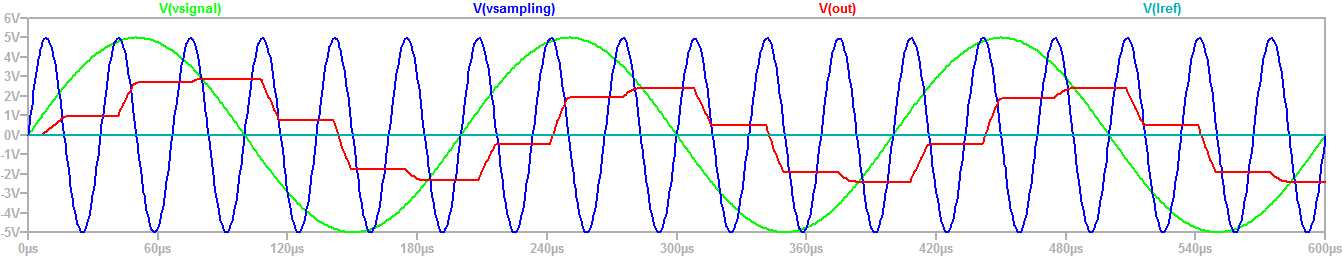
\includegraphics[width=\linewidth]{ImagenesEjercicio4/ChTests/Vin1_30ksamplig47nF}
	\caption{Sinusoidal 5KHz muestreada a 30KHz con un $C_{hold}=47nF$}
	\label{fig:vin130ksamplig47nf}
\end{figure}
En color \textcolor{red}{rojo} observamos el resultado de la operación de muestreado. 
Cuando la señal de muestreo, en \textcolor{blue}{azul}, supera el nivel de la tensión de lógica de referencia(\textcolor{turquoise}{turquesa}), en este caso seleccionada en 0V, la llave "se cierra" y comienza el proceso de muestreo. Esto implica que el capacitor, $C_{hold}$, puede comenzar a cargarse con el valor que tenga señal de entrada durante el tiempo que permanezca en ese modo. Cuando la señal de muestreo se encuentra por debajo de la tensión lógica de referencia se ingresa al modo \textbf{hold}, la llave "se abre" y el capacitor retiene el último valor obtenido. No obstante vemos que la el valor de tensión almacenado en el capacitor no consigue equiparar aquel de la señal a muestrear. Recordemos que entre mayor sea el valor de la capacitancia más tiempo tardara en cargarse, lo cual afecta el desempeño en el modo de muestreo pero mejora significativamente la persistencia durante el tiempo de \textbf{hold} ya que por el contrario tarde más en cargarse.

En este caso se hace evidente que el capacitor no consigue cargarse lo suficientemente rápido.

\begin{figure}[H]
	\centering
	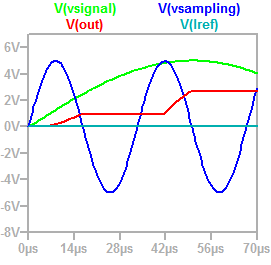
\includegraphics[]{ImagenesEjercicio4/ChTests/Vin1_30ksamplig47nFZoom}
	\caption{Vista en detalle del proceso}
	\label{fig:vin130ksamplig47nfzoom}
\end{figure}

Para poder exhibir el caso opuesto se utilizo un capacitor $C_{hold}$ de $120pF$. Este capacitor posee una capacitancia aproximadamente 400 veces más pequeña que la utilizada anteriormente.
En este caso la señal de salida representa más fielmente a la original. Una primera observación nos deja observar que los valores de tensión obtenidos durante el muestreo  

\begin{figure}[H]
	\centering
	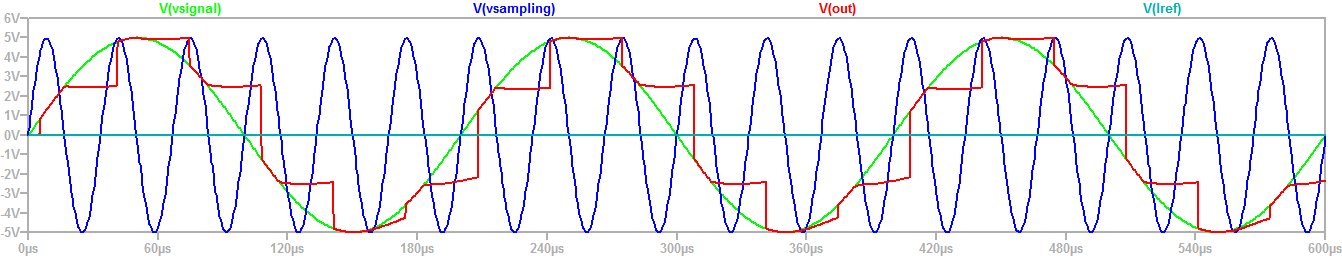
\includegraphics[width=\linewidth]{ImagenesEjercicio4/ChTests/Vin1_30ksamplig120pF}
	\caption{}
	\label{fig:vin130ksamplig120pf}
\end{figure}


\begin{figure}[H]
	\centering
	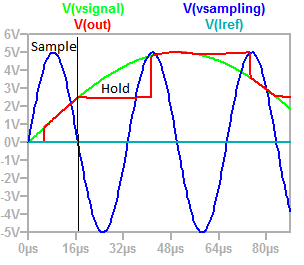
\includegraphics[]{ImagenesEjercicio4/ChTests/Vin1_30ksamplig120pFZoom2}
	\caption{}
	\label{fig:vin130ksamplig120pfzoom}
\end{figure}


Analizando la figura \ref{fig:vin130ksamplig120pfzoom} notamos que el capacitor efectivamente consigue cargarse lo suficientemente rápido como para poder seguirle el paso a la señal de entrada. 


Ahora veremos lo que sucede cuando empleamos una señal más rápida.
La señal senoidal ahora posee una frecuencia de oscilación de $20*3*12 KHz = 720KHz$. Para poder obtener imágenes y apreciar los cambios en los capacitores elegidos es necesarios muestrear a la señal por encima de la mínima permitida por el criterio de Nyquist. Sin embargo, si consideramos ese caso obtenemos  $F_{nyqusit}=1.44Mhz$.
Para la simulación de la  figura \ref{fig:vin21440ksamplign120pf} se utilizo el capacitor de $120pF$ que había obtenido buenos resultados previamente. Pese a ello una imagen poco anticipada aparece al finalizar la simulación. La salida parecería ser nula. Aun si esta no fuese nula no sirve a nuestros propósitos. 
\begin{figure}[H]
	\centering
	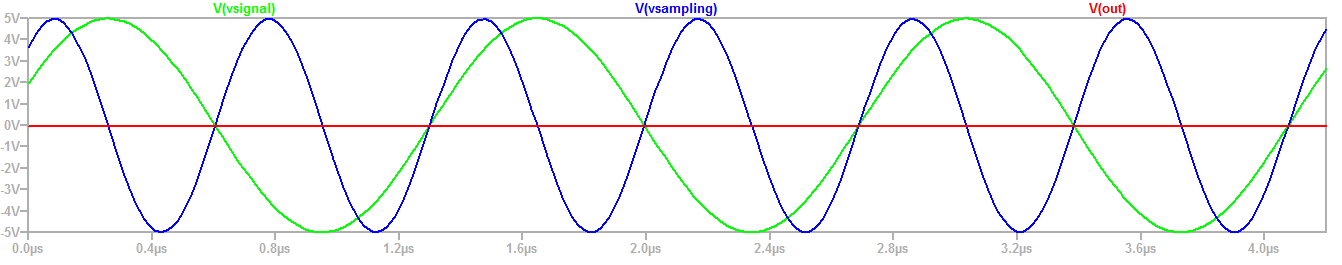
\includegraphics[width=\linewidth]{ImagenesEjercicio4/ChTests/Vin2_1440kSamplign120pF}
	\caption{}
	\label{fig:vin21440ksamplign120pf}
\end{figure}

Entonces cabe preguntarse que ha sucedido aquí. 
En primer lugar podemos relacionar lo ocurrido aquí con lo sucedido cuando se utilizo un capacitor demasiado grande que no conseguía cargarse en la ventana de adquisición provista y por lo tanto exhibía una amplitud menor.

\begin{figure}[H]
	\centering
	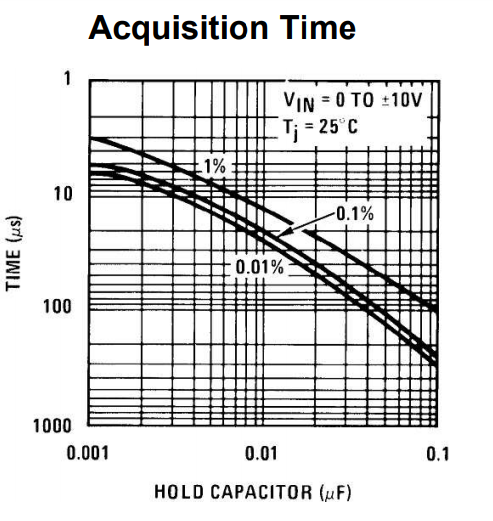
\includegraphics[scale=0.6]{ImagenesEjercicio4/HoldCapAcqTime}
	\caption{}
	\label{fig:holdcapacqtime}
\end{figure}

Si elegimos muestrear a la frecuencia de Nyquist entonces le estamos dando al $C_{hold}$ un tiempo de $T_{acq}=\frac{1}{2*F_{nyquist}}$
$$T_{acq}\approx 700ns = 0.7\mu s$$
Por lo tanto, si hacemos referencia a las curvas de la figura \ref{fig:holdcapacqtime} vemos que nuestro requerimiento esta por fuera de las capacidades del \textbf{LF398}. En conclusión, necesitaríamos capacitancias extremadamente pequeñas. Lo cual tiene como contrapartida que no podrán mantener el valor almacenado durante mucho tiempo.
\subsubsection{Elección del $C_{hold}$ apropiado}
Como analizamos anteriormente, es de suma importancia elegir un capacitor que se cargue lo suficientemente rápido como para poder seguir a la señal de entrada y que a su vez pueda retener el valor muestreado sin degradarse. 
En nuestro caso de aplicación se sabe que la señal de control tendrá una frecuencia máxima de $F_{osc}=25KHz$. Por lo tanto el capacitor de hold tendrá un tiempo de adquisición mínimo dado por:
$$T_{acq}=\frac{1}{2*F_{nyquist}}\approx20\mu s$$

Entonces observando la figura debajo tenemos 3 opciones a elegir dependiendo de que tan preciso queramos y/o necesitemos que sea el valor de la muestra. Esto se debe a que la elección del capacitor nos lleva a una relación de compromiso. Podemos reducir el tiempo de adquisición al elegir un capacitor más pequeño pero esto incrementara el \textbf{hold step} y el \textbf{droop rate} lo cual puede ser contraproducente.

\begin{figure}[H]
	\begin{subfigure}[b]{0.4\linewidth}
		\centering
		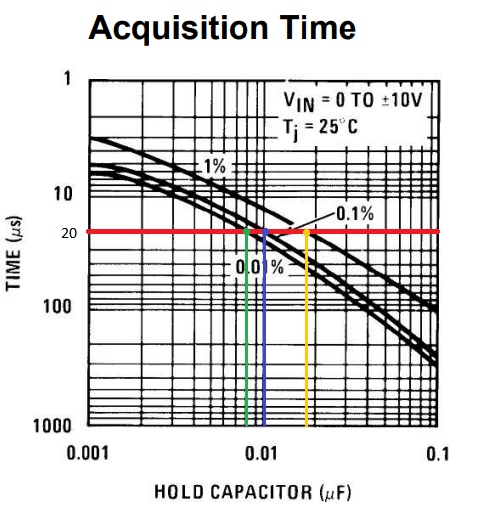
\includegraphics[scale=0.6]{ImagenesEjercicio4/HoldCapAcqTimeSl.png}
		\caption{}
		\label{fig:holdcapacqtimeSL}
	\end{subfigure}
	~
	\begin{subfigure}[b]{0.4\linewidth}
		\centering
		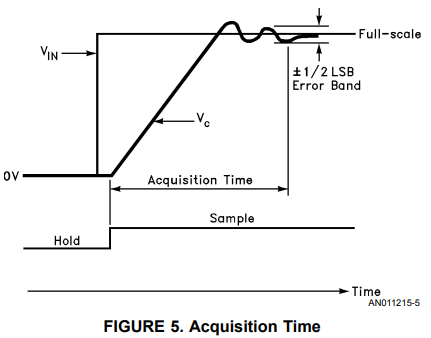
\includegraphics[]{ImagenesEjercicio4/AcqTime.PNG}
		\caption{}
		\label{fig:acqtime}
	\end{subfigure}
 \caption{\ref{fig:holdcapacqtimeSL} Capacitor de Hold en función del tiempo de adquisición. \ref{fig:acqtime} Vista en detalle del muestreo y los efectos del Hold Step}
\end{figure}


\begin{table}[H]
	\centering
	\begin{tabular}{@{}lrlll@{}}
		\toprule
		\multicolumn{1}{c}{\textbf{Error \%}} & \multicolumn{1}{c}{\textbf{C}} &  &  &  \\ \midrule
		0.01                                  & 8nF                            &  &  &  \\
		0.1                                   & 10nF                           &  &  &  \\
		1                                     & 16nF                           &  &  &  \\ \bottomrule
	\end{tabular}
	\caption{Valores de capacitor posibles según el error aceptado}
	\label{tab:acqCap}
\end{table}
	
Dadas estas 3 opciones ahora debemos también considerar el \textbf{hold step}. Este fenómeno se describe como un escalón de tensión que es generado cuando se pasa de modo \textit{sample} a modo \textit{hold}.
\begin{figure}[H]
	\centering
	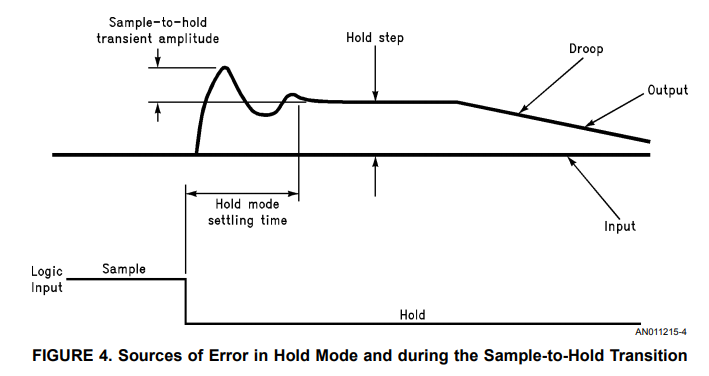
\includegraphics[scale=0.6]{ImagenesEjercicio4/HoldStepError}
	\caption{Vista en detalle de los efectos del hold step}
	\label{fig:holdsteperror}
\end{figure}

Siguiendo las recomendaciones del fabricante, es deseable que el \textbf{hold step} se mantenga por debajo de la mitad del paso de tensión que representa al LSB. Asumiendo un que los rangos de señal pueden variar entre $\pm15$ nos da una $FS=30$.
$$V_{hs}<\frac{FS}{2^{n+1}}$$
$$V_{hs}<\frac{30V}{2^{8+1}}$$

$$V_{hs}< 58.5mV$$

En la figura a continuación denotamos dónde se encuentra este limite de forma aproximada. 
\begin{figure}[H]
	\centering
	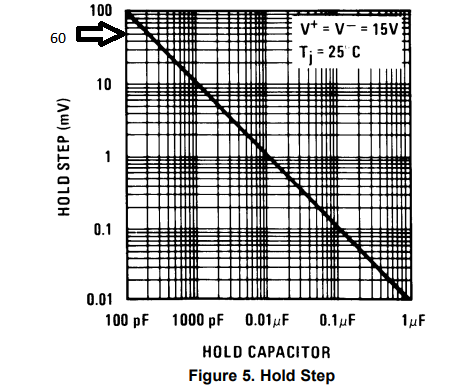
\includegraphics[scale=0.7]{ImagenesEjercicio4/HoldStepMarcado}
	\caption{}
	\label{fig:holdstep}
\end{figure}

Esto quiere decir que podemos movernos hacia abajo en la curva con bastante libertad dado que cualquier valor de capacitor por encima de los $110pF$ respetara el limite de $V_{hs}$ impuesto.\\
Por ultimó debemos tener en cuenta la tecnología de capacitor a utilizar.
\begin{figure}[H]
	\centering
	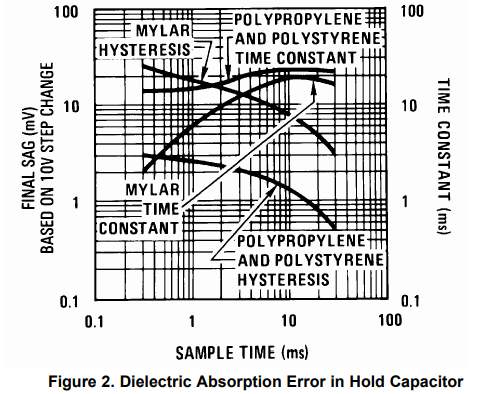
\includegraphics[scale=0.7]{ImagenesEjercicio4/AbsorcionDielectrico}
	\caption{}
	\label{fig:absorciondielectrico}
\end{figure}
La figura \ref{fig:absorciondielectrico} nos indica como cambia la histeresis de diferentes capacitores según el tiempo de muestreo. En una primera observación el gráfico puede resultar un poco confuso. Recordemos que el $T_{acq}=20\mu s$ y la escala horizontal tiene unidades de $ms$. Esto es porque las curvas intentan comunicar que tan bien consiguen relajarse los capacitores luego de realizar un muestreo de tal forma que no quede un remanente que afecte a la siguiente muestre.
La importancia de elegir el tipo correcto de tecnología impacta sobre el \textbf{droop rate} y en al precisión del muestreo. Se comparan dos grandes grupos de tecnologías, por un lado los capacitores \textbf{Mylar} (film)

Por lo expresado anteriormente se utilizara un capacitor de $C_h = 8nF$ dado que nos ofrece el menor error de muestreo y mantiene las exigencias dadas por el \textit{hold step}

Dadas las curvas y las recomendaciones del fabricante se utilizaran capacitores de poliestireno dada su baja histeresis.

\subsubsection{Analizando otros modelos de Sample and Hold IC}
Por lo general los módulo de Sample and Hold vienen ya incorporados dentro de los \textbf{ADC} por lo que no hay abundancia de modelos en el mercado. Sin embargo, esto no quiere decir que el \textbf{LF398} sea el único. En esta ocasión vamos a compara al \textbf{LF398} contra el \textbf{SMP04} de \textit{Analog Devices}
% Please add the following required packages to your document preamble:
% \usepackage{booktabs}
\begin{table}[H]
	\centering
	\begin{tabular}{@{}lll@{}}
		\toprule
		& \textbf{LF398}                & \textbf{SPM04}                  \\ \midrule
		Impendancia de entrada                     & 10G$\omega$                   & No posee
		Input Buffers      \\
		Tiempo de adquisición con error de  0.1 \% & \multicolumn{1}{r}{4 $\mu$ s} & \multicolumn{1}{r}{3,5 $\mu$ s} \\
		$C_h$ Interno                              & \multicolumn{1}{r}{NO}        & \multicolumn{1}{r}{YES}         \\
		HOLD step (similar test condition)         & \multicolumn{1}{r}{2 mV}      & \multicolumn{1}{r}{2,5}         \\
		Tensión de Offset de entrada Typ           & $\pm$ 2mV                     & $\pm$ 2,5mV                     \\
		Tensión de Offset de entrada Max           & $\pm$ 7mV                     & $\pm$ 10mV                      \\ \bottomrule
	\end{tabular}
	\caption{Tabla comparativa del LF398 de Texas Instruments vs SMP}
	\label{tab:sampleandholdcomparisson}
\end{table}

No poseer buffers de entrada presupone una gran desventaja frente al \textbf{LF398} dado que esto nos limita los tipos de fuentes de señal que podemos colocar a la entrada. Por el contrario la gran impedancia de entrada en el IC fabricado por TI conseguimos total independencia de la impedancia de salida de la fuente de señal y por lo tanto mitigamos los efectos de carga del sample and hold sobre la fuente preservando la información contenida en la señal.  
El \textbf{SPM04} presenta una mayor tensión de offset, esto puede forzar al diseñador a implementar alguna solución para compensar esta magnitud en caso de que produzca errores significativos dependiendo de las condiciones de uso. Sin embargo, a diferencia de Texas Instruments, Analog Devices no propone ningún circuito de compensación ni pines adicionales para implementarlo. 
Haciendo un paralelo entre ambas hojas de datos, podemos afirmar que es bastante complicado conseguir compararlos debido a las diferentes condiciones de prueba bajo las que fueron sometidos. 


%\end{document}